\section{OpenGL rendering process} \label{sec:opengl-rendering}
In order to obtain good renderings for training and recognition purposes, it is
important to create photo realistic, virtual snapshots of the objects in
diffent poses. It is also important to use the same model of camera introduced in sec.
\ref{sec:camera_modelling} in the most uniform manner as possible.

In this section, this modelling is described. First, a brief
introduction to OpenGL (sec. \ref{sec:opengl-intro}) and to the correct usage of homogeneous coordinates (sec.
\ref{sec:homogeneous-coordinates}) is done, followed by a description of OpenGL reference systems (sec.
\ref{sec:opengl-reference-systems}). After this, the OpenGL rendering
process is analyzed more in details (sec. \ref{sec:opengl-rendering-process}), and finally the
implementation of objects' rendering for the purpose of this project is
described keeping all of the previous into account (sec. \ref{sec:renderer3d}).

\subsection{OpenGL graphics library} \label{sec:opengl-intro}
OpenGL\footnote{www.opengl.org} is a free (GPL) software interface to graphics hardware \cite{opengl-book}. This
library allows a programmer to build incredibly complex, interactive 3D graphics
applications (a lot of modern PC games are an example) without the need of
directly interfacing the graphics hardware, which in most of cases has an
extremely complicated architecture and variegated set of features. Instead, a
set of standard 3D graphics functions (\emph{API}) for the C programming
language is exposed to the developer, and the hassle of linking these
functions to the hardware is left to the manufacturer, who will provide its own
optimized implementation of the library together with the hardware.

Being industrial-level free software, this library has become very popular, and
well-working implementations exist for most of the modern graphics hardware
available nowadays. Also, it is highly portable (stripped-down versions of OpenGL
called \emph{OpenGL-ES} exist for embedded systems and systems with limited
resources in general, such as Android mobile phones); in this sense, OpenGL is
a perfect fit for image processing systems requiring a 3D rendering feedback to
work, like this one, in order to be easily ported and implemented in real-world
applications.

As a 3D graphics engine, and considering that it targets a wide range of devices, OpenGL only manages simple primitives' rendering, such
as points', lines' and polygons'. It does \emph{not}, thus, implement
high level tasks like window management or user input, which may be not even
available on the system the application's running onto.

However, a set of various complementary libraries exist, which can be used in
synergy with OpenGL to provide such functionalities. The ones used during the
course of this project are:

\begin{itemize}
  \item{\emph{The OpenGL Utility Toolkit
      (\emph{GLUT})}\footnote{https://www.opengl.org/resources/libraries/glut/} a
      nonfree library, written by Mark Kilgard to support its OpenGL guide
      \cite{opengl-book}, tightly bundled to OpenGL and
      almost always shipped together with it, which helps the programmer in all the
      aforementioned tasks. In particular, it provides a cross-platform abstraction
      for window creation and management, and for user event handling; it also
      provides the programmer with high-level shape creation routines. A free
      implementation and extension called
      \emph{FreeGLUT}\footnote{http://freeglut.sourceforge.net/} exists and is used
      worldwide as a replacement for GLUT, as the last version (3.7) of the latter dates
      back to
    1997;\footnote{http://www.ibiblio.org/pub/packages/development/graphics/glut/}}

  \item{
      \emph{Open Asset Import Library (\emph{Assimp})}, which is a support library which
      can be used to import various mesh formats into a uniform, object-oriented (C++)
      data structure. It is useful to generate at runtime a vertex list and rendering
      data for objects
      generated from external data, such as the objects' models used into this project
      for object recognition purposes.
    }
\end{itemize}
\subsection{Homogeneous coordinates} \label{sec:homogeneous-coordinates}
Homogeneous coordinates were introduced by the famous mathematician August Ferdinand Möbius in
\cite{homogeneous-coordinates}; they are a common way to represent points in
\emph{projective geometry} by using an additional scale value, usually called
$w$, in represented
vectors, which can be seen as an inverted scale factor for the whole vector. In
practice this means that the association between homogeneous coordinates $H$ and
cartesian coordinates $C$ is:


\begin{equation}
H=\left(\begin{array}{c}wx\\wy\\wz\\w\end{array}\right) \Leftrightarrow
C=\left(\begin{array}{c}x\\y\\z\end{array}\right)
\end{equation}

Although this generates redundancy, as there will always be more freedom degrees
then constraints when mapping from coordinates to points (2D points are
represented with 3 values, 3D points with 4, and so on), this notation can
simplify a lot the computing effort for usual geometric operations -- for
example, scaling a set of points only requires to change their $w$ value.
Also, when performing matrix operations, this geometry has the good property to
be \emph{scale-invariant} for vectors, which means that coordinates are
multiplied by a constant value they keep representing the same point.

The last interesting property of homogeneous coordinates for the purposes of
this thesis is their capability to easily distinguish points from directions;
in fact, a directional vector can be represented as a point at the infinity,
and, differentely from cartesian coordinate systems, homogeneous coordinates
easily represent them as directional vectors by setting their $w$ coordinate to
$0$.

Also, \emph{all} affine transformations, if operating on homogeneous
coordinates, can be representing as $4\times 4$ matrices including rotation
matrix $R$, translation vector $T$, and scale properties $s$:

\begin{equation}
  A=\begin{pmatrix}
    R & T \\
    0 & s
  \end{pmatrix}
\end{equation}

By representing directional vectors as points at the infinity, they will have
the good property of never being scaled nor translated by these transformation,
which is desirable e.g. for unit direction vectors.

OpenGL, together with applications like OpenCV and algebraic libraries like
Eigen\footnote{eigen.org}, use homogeneous coordinates for almost all of their
work. During this project, homogeneous coordinates have been used extensively
thanks to the Eigen library, in order to have a well-defined system (Affine
transformations) to define the reference systems of interest, and in order to
compute transformations between objects. Homogeneous coordinates are converted
to native formats (e.g. COMAU robots' euler axis representation) only in the
final backend of the applications, so that data representation is unique and
coherent in the whole scope of the project.

\subsection{OpenGL reference systems} \label{sec:opengl-reference-systems}
Opposing to a lot of 3D manipulation systems, such as COMAU's robotic arms or
CAD applications, which use different coordinate systems for different logical
aspects of their work, typically requiring at least a \emph{local} and a
\emph{global} coordinate system, OpenGL only works with a single 
coordinate system (\emph{clip coordinates}) when drawing (rendering) objects,
in which camera's frame is fixed at the origin and aligned with global axes,
with Z-axis pointing backward\footnote{This actually brings out a left-handed
  coordinate system, which must be taken into account when interfacing OpenGL
with external world like it has been done in this project.},
which is then transformed into another unique coordinate system
(\emph{Normalized device coordinates}) after drawing in order to map 3D points to 2D points into the
render (camera) buffer. A third buffer (\emph{Z-depth buffer}) keeps
informations about the depth of drown points into the visible scene and is
registered with the rendering buffer. As described in \cite{opengl-book}, in order to give the
programmer full access capabilities to the rendering engine's internals, 
multiple reference systems appear to the user only on the
OpenGL API's abstraction layer, in which different functions \emph{appear} to
work on different coordinate systems, but instead limit themselves to act
differently on the latter. Thus, with the target of emulating a physical
camera in mind, the programmer can act on the most suitable components of the
rendering process as needed, without caring about what is the right coordinate
system to transform. 

\subsection{Details about OpenGL rendering process} \label{sec:opengl-rendering-process}
Here follows a description of the full process performed by OpenGL in order to
render a 3D mesh, from scene generation to actual mapping of 3D points into a
2D buffer. A complete and detailed description can be found in
\cite{opengl-book}, completed of actual API examples which are omitted here
for brevity.

OpenGL library implements a state machine: sequential calls to library
functions modify internal state variables (e.g. colour information), allowing the renderer to be
instructed about how to add elements in the scene and how to transform them to
get the final renderer. Thus, single, independent objects can draw themselves
into the scene and manage each one a single part of the scene (e.g. camera and
fog): current scene's state is actually a global accessible datum. While this
has the obvious advantage of full and deep freedom of implementation, it also
brings the drawback of needing to be careful for how each of the elements
modifies the global state when it finishes operating. In general, it is thus
important to define with extreme precision what each object is supposed to do
and never implement complex operations in a single block, rather splitting them
into single, well-defined tasks.

In this project the simpler -- although deprecated in newest (3.0) versions and
substituted by shaders --
rendering procedure using OpenGL's \emph{fixed pipeline} has been used; this
procedure assimilates the rendering process to an assembly line, in which every
element of the scene undergoes a predefined sequence of processing steps before
being merged with others to form the final render. In particular, geometric data
like lines or polygons are moved into the scene, cut based on their $z$ coordinate, and
finally mapped to 2D screen coordinates through the \emph{projection matrix}.
Mapped points are then bound to 2D data like bitmaps and 2D points in a
process called \emph{rasterization}; finally, every token can be modified by
\emph{per-fragment operations}, like texture appliances and alpha (transparency)
computation.

The first operation done by the renderer is taking the list of vertices
which have to be drown from the global state. Vertices can be added to the
scene by use of \emph{display list} (cached sets of 3D vertices created using
basic drawing functions) or explicitely drown during a single rendering
iteration. Drawing primitives different from vertices, which were inserted into a
display list via drawing functions, are numerically computed and transformed to
vertices sets too.

From vertices informations OpenGL extrapolates geometric primitives'
data, like surfaces, edges, texture coordinates.
Each primitive is then moved into the scene through an affine transformation
described by the \emph{Modelview matrix}. This $4 \times 4$ matrix multiplies
each primitive on the left to produce its coordinate in the first of two
coordinate systems described in sec. \ref{sec:opengl-reference-systems}, called
\emph{clip coordinates}. This is the global, 3D reference system and is the one in
which the actual 3D drawing is done: first, $z$ coordinate is used to determine
which parts of which object will actually be visible. Points are not considered
if their $z$ coordinate makes them covered by another object. At this point the
whole scene is clipped (hence the name), using two planes, \emph{near} and
\emph{far} clipping planes. Objects are kept if they lie in between this planes,
i.e. if and only if $near<z<far$ as shown in fig. \ref{fig:clipping-planes}.
This is to minimize the number of objects to process, by removing objects that
are actually too far away or too near to be rendered accurately. These values
must be chosen in the most restrictive way as possible: this is because $z$
coordinate is mapped to its output buffer (depth buffer) with a low-range
(usually, $12\unit{b}$) value, taking the values of $near$ and $far$ as a
reference for minimum and maximum value. So, having a too wide range in near and
far planes results in heavy loss of depth information due to discretization of
depth values.

\begin{figure}[htbp]
  \centering
  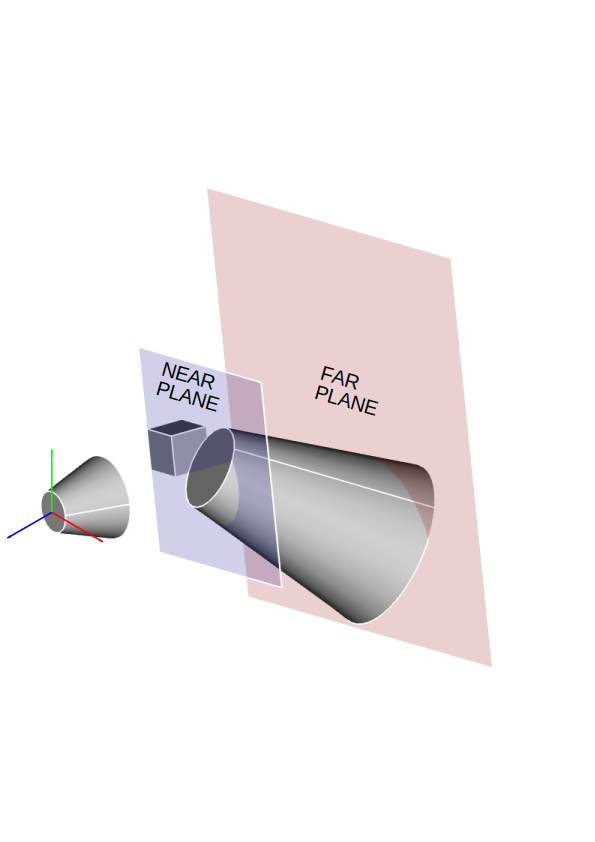
\includegraphics[width=4in]{./Graphics/clipping_planes}
  \caption{Defined into the camera's coordinate system (left), the near and far clipping planes are used to minimize the number of
  primitives to process, as well as reference points for depth computation. \label{fig:clipping-planes}}
\end{figure}

Raw colouring information in applied at this stage and primitives are finally
mapped into screen by a second $4\times 4$ matrix, the \emph{perspective
matrix}. At the end of this process objects are said to be in \emph{normalized
device coordinates \emph{NDC}}. In NDC, the (virtual) cube spawning the
$\left(-1,1\right)$ range in each direction is projected orthographically on the
output image buffer (considering $x$ and $y$ coordinates), with each corner
corrisponding to an angle of the window (called \emph{Viewport}) -- top, bottom,
right, left-- and depth buffer
(mapping the $(-1,1)$ $z$ coordinate to the range $\left( near , far \right)$ as described
before).

Finally, texture information in form of \emph{texels} (texture elements) is applied to primitives if needed and other
processing such as fog calculation is done. The image is completely rendered at
this point and can be accessed via direct reading from raw data buffers.

\subsection{Antialiasing of polygons and textures} \label{sec:antialiasing}
\label{sec:FBO}
%TODO antialiasing of textures
During the last phase of rendering, OpenGL's pipeline silently associate each
pixel primitive, with its matching texture and depth information, with a single
colour (RGB) and depth value (alpha). If only the geometric information relative
to the center of the pixels is considered (as done by default), this will cause
high rendering quality degradation: this is because contours of objects and
textures will be neatly mapped on a per-pixel basis, and so their lines --
especially if almost vertical or almost horizontal -- will appear more as a
polyline than a single, straight line. This effect is shown in fig.
\ref{fig:polyline}. To solve this issue, a set of techniques for what is called
\emph{antialiasing} are implemented. If implemented correctly, antialiasing of
polygons' edges and texture data can improve image quality by blending the
boundaries between adjacent polygons, thus providing a more photorealistic
render.

\begin{figure}[htbp]
  \centering
  \includegraphics[width=2.5in]{./Graphics/antialiasing}
  \caption{A 1-pixel line generates rough boundaries on when rendering on a
  per-pixel basis. Multisample antialiasing can solve the problem by
approximating the line as a 4-pixel rectangle and averaging each multisampled
pixel with its neighbours. \label{fig:polyline}}
\end{figure}

Old versions of OpenGL provided a set of features called \emph{smoothing}, which
emulated transparency (alpha) value on pixels on the border in order to blend
them with neighbour pixels. Newer versions have deprecated this techniques in
place of \emph{Multisampling}. By using multisampling, each pixel primitive --
as the one obtained after the rasterization process -- is actually splitted in
four or more parts into a special, offscreen buffer, and the image is treated as
it was a render with higher resolution, except for coordinate systems which will
be left untouched -- so that the entire process is transparent to the
programmer. After rendering, the offscreen buffer is copied to the result buffer
and is said to be \emph{resolved}: in this stage, each pixel is formed by
averaging the content of the four micro-pixels which compose it. Multisampled
has been preferred over smoothing because, although requiring a lot of memory
for storing the high-resolution image -- which is not a problem with modern
graphics hardware as it was when smoothing was born --  it provides both faster
performance and better quality, as explained in \cite{opengl-book}.

The special buffer for offscreen rendering is implemented in OpenGL through the
means of a \emph{Framebuffer object (\emph{FBO})}.
Framebuffer objects are special drawing buffers, introduced with OpenGL 3.0,
which emulate a real framebuffer (i.e. the are of a video memory which
the software will draw onto), keeping the allocated memory area totally
independent from the actual video memory of the rendering window. Apart from
their physical location, they look totally equivalent to a normal rendering
window, and just like it they have a set of buffers to which the application can
draw, the main ones being the color and depth buffer. These can be bound 
at runtime to a physical location in memory by assigning (\emph{plugging}) new buffers to the \emph{attachment point} of a
framebuffer. A framebuffer can be drawn onto if and only if it is
\emph{complete}, i.e. if all its main attachment points (colour and depth) have
been bound to a physical buffer.

Apart from multiple uses which are irrelevant for this project (like dynamically
updating a texture by offscreen rendering onto it), the main scope of FBOs is
their multisample capabilities. In fact, it is sufficient to plug
multisample-capable buffers (which can be generated using OpenGL's allocation
functions) to the colour and depth attachment points of an FBO and select the
latter as the default rendering buffer to have the application draw all of its
raster data there, thus keeping multisample into account. 

When the final render has to be read, however, it is not sufficient to read the
raw drawing buffer from the FBO, as it has a totally different internal
structure in order to keep track of the needed geometric transformations needed
not to change the geometry's position despite of multisampling. A special
function, called \emph{blitting}, can be used to copy the multisampled data to
another framebuffer, allocated with raw RGB pixels and thus capable of being
read with the expected result. When blitting is applied to the multisampled
framebuffer, it is automatically resolved to pixels; in this way, the resolved
buffer can be copied byte-per-byte into the raw FBO.

Texture multisampling is also implemented with this method and provides a good
result. However, for textures the situation is different as also another factor
must be considered: as the object reduces
its dimensions, texture internal data will be dropped during the mapping from 3D
to 2D coordinate, because it actually is applied on a per-2D-pixel basis during the
last stage of rendering (after rasterization has been done), as depicted in sec.
\ref{sec:opengl-rendering}. This process downsamples heavily the texture -- even if
polygon multisampling is enabled -- as no interpolation is done when scaling
down the texture for appliance.

To solve this issue, OpenGL allows the programmer to specify a set of textures
of different size for the same object. Element of this set, which can be easily
generated automatically starting from the biggest texture, are called
\emph{mipmaps}. At the 2D texturing stage, OpenGL will choose the correct image
to map points to, and $(u,v)$ coordinates on it, based on a \emph{strategy}
which can be defined at runtime. Simpler strategies assume for example to always
take the first texture which is bigger or smaller than the primitive to cover,
while more complex ones allow to refine the result at expense of a bigger
computing time, by linearly interpolating between these two textures to produce
a middle texture component.

As said in sec. \ref{sec:opengl-intro}, OpenGL tends to be extrimely frugal in the
number of implemented features: the only supported method for adding mipmaps to
a texture is manually adding a series of differently sized images to the texture
data. As it is quite easy to generate this data automatically and with good
quality, however, the GLUT library exports useful functions to automatically
build the set of textures of increasing size and adding them to the texture.
A native extension for OpenGL allows to generate mipmaps when and only when
needed, at the cost of random loss of GPU cycles into the program; this extension is,
however, only present in newest versions of OpenGL and is not supported by some
graphic hardwares (e.g. Intel HD4000). The programmer must explicitely check for
its presence, and only when the extension is found by OpenGL he can safely
assume that no manual (or semi-automatic) mipmap generation is needed.

Texture mipmaps allow a 3D rendering application to reduce at its minimum the
number of discarded of data due to texture downsampling: instead, they allow to
produce high-quality, low-sized images when initializing the system (i.e. when
the program can afford to lose time to produce this data using complex filters
such as cubic interpolation). The visual result of texture mipmapping is
qualitative relevant and can be observed, together with the effect of
multisample on geometry, in fig. \ref{fig:multisampling-on}

\begin{figure}[htbp]
  \centering
  \includegraphics[width=2.5in]{./Results/antialiasing}
  \caption{Rendering with antialiasing and mipmapping on (left)
  can improve a lot the quality of the result with respect to the same options
turned off (right). \label{fig:multisampling-on}.}
\end{figure}

\section{Implementation of objects' rendering} \label{sec:renderer3d}
With the details explained in sec. \ref{sec:opengl-rendering} in mind, a mesh renderer has been implemented, capable of
reading objects' meshes from files as needed; together with meshes, it reads the full model of
camera with which training has to be done, and renders them in the required
pose, also extrapolating useful informations from the render which can be used
for training. All the interface of the renderer with the external world is done
using the conventions of the whole project: cameras are modelled using OpenCV's
standard reference systems and calibration matrices described into sec.
\ref{sec:camera_modelling}, while object poses are described as affine
transformations acting on homogeneous coordinates as in sec.
\ref{sec:homogeneous-coordinates}. At time of objects' creation, the Assimp library
is used to convert the mesh file, in whichever format it is, into Assimp's
unified structure, which for simplicity's sake can be simplifiethought of as a tree of
nodes, each representing a face, a texture to be applied to children, or
an affine transformation to be applied to children. When the renderer is created
it configures itself using GLUT to open a window and create the RGB and depth
framebuffers in which to render. Renderer's initialization is a one-time
operation, and is performed statically by the first object using GLUT. During
this phase, renderer also initializes the needed parameters for multisampling as
described in sec. \ref{sec:antialiasing}.

Three main features have been implemented, which can be used as an access point
to the renderer: the first one can set the
camera model by reading it from the project's camera data structure; the second
one can set the reference position of objects into camera's space (in this project's
conventions, i.e. in OpenCV not in OpenGL one); the third function can render a
mesh and extract RGB and depth buffers to OpenCV matrices for later use. This
last feature also extracts object's bounding box information and rendering mask,
which will be used for training and recognition filtering in sec.
\ref{sec:vision}.

\subsection{OpenGL camera modelling}
The goal of the first set of functions of the renderer is to interface OpenGL's
projection system with the global camera models used into the project; in
OpenGL camera's parameters are not defined and only a single matrix is used to
transform 3D coordinates in camera frame to 2D points onto the image. Keeping in
mind the definitions of intrinsic parameters of the camera, as described in sec.
\ref{sec:intrinsics}, this is accomplished into three steps.

First, the intrinsic matrix of the camera is extracted from the
camera's model, and from it the relevant camera parameters are read.

From this data, the projection matrix 
\begin{equation}
  M_{\text{int}}=\begin{pmatrix}
    f_x & 0 & -c_x & 0\\
    0 & f_y & -c_y & 0\\
    0 & 0 & (N+F) & NF \\
    0 & 0 & 0 & -1 
  \end{pmatrix}
\end{equation}

is built. This matrix is similar to the camera intrinsic matrix, but with two
main differences: first and most important, it operates on 3D points (in clip
coordinates) producing
other 3D points. If applied to a point, $x$ and $y$ coordinates in output are the same as they would be
if mapped using intrinsic matrix, but $z$ coordinate is mapped to the $near-far$
range. Second, the Z axis points forward in our convention, backward in OpenGL.
Thus the matrix is built so that the Z coordinate will be inverted while
preserving X and Y.

After this, clip coordinates have been transformed in what would are OpenCV's
camera coordinates, plus $z$. In order to port them into OpenGL's NDC, another
transformation is needed, which simply scales the view range (\emph{view
frustrum}) to linearly fit the NDC:

\begin{eqnarray}
  L = x_{\text{left}} & = & 0 \nonumber \\
  R = x_{\text{right}} & = & W_{\text{cam}} \nonumber \\
  B = y_{\text{bottom}} & = & H_{\text{cam}} \nonumber \\
  T = y_{\text{top}} & = & 0 \nonumber \\
  M_{\text{fit}} & = & 
  \begin{pmatrix}
    \frac{2}{R-L} & 0 & 0 & -\frac{R+L}{R-L} \\
    0 & \frac{2}{T-B} & 0 & -\frac{T+B}{T-B} \\
    0 & 0 & -\frac{2}{F-N} & -\frac{F+N}{F-N} \\
    0 & 0 & 0 & 1
  \end{pmatrix}
\end{eqnarray}

The two matrices are multiplied to get the final projection matrix, which is
passed to OpenGL as the matrix which maps clip coordinates to NDC:

\begin{equation}
  M_{\texttt{proj}}=M_{\text{fit}}M_{\text{int}}
\end{equation}

Also, OpenGL is instructed to which pixels and depth ranges correponds to the
NDC by setting its \emph{viewport}, \emph{near} and \emph{far} values.

At the end of this process, OpenGL will thus map automatically points in global
3D space with points in camera frame.

\subsection{Object movement into global space}
Into the project's convention, each object has got its own local coordinate
system, and the mesh is built with all its verteces into this system,with all
its verteces into this system,  as explained into sec. \ref{sec:cad-mesh}. Every
object is then stored into its mesh file as if it was centered into the global
origin. Assimp library is used to read this mesh file and produce a set of faces
together with their vertices' coordinates. From the external world, however, the global
renderer can display a mesh into a specified pose in the global coordinate
system obeying the specifications of the project. This system is different from
OpenGL's one, which only knows camera (clip) coordinates. In order to move
the object from the global system to the right position in OpenGL reference
system the \emph{Modelview} matrix is used: this will be automatically applied
to OpenGL when drawing each primitive, and will modify its coordinates
accordignly. In order to take into account the difference between the global
coordinate system and OpenGL's clipping coordinates, a $\pi$ rotation along the
$X$ axis is applied
to the Modelview matrix \emph{before} the actual pose, which as usual is
already represented as a $4 \times 4$ affine transformation matrix:

\begin{equation} \label{eqn:modelview}
  M_{\text{modelview}} = 
  \begin{pmatrix}
    1 & 0 & 0 & 0 \\
    0 & -1 & 0 & 0 \\
    0 & 0 & -1 & 0 \\
    0 & 0 & 0 & 1 
  \end{pmatrix} M_{\text{pose}}
\end{equation}

Another convenience function is presented to the user, which can emulate
camera's movement around the object: in this case, the object's pose is first
computed as the inverse of camera pose ($M_{pose}=M_{cam}^{-1}$), and it is
finally applied as in eqn. \ref{eqn:modelview}.

\subsection{Object rendering and image processing} \label{sec:meshdraw}
When all the rendering parameters has been set accordingly to the desired scene
parameters and emulated camera model, the renderer can be asked for to finally
get the rendered image of a mesh object. When done, it is actually the mesh that
renders itself into the OpenGL's framebuffer. As the mesh knows its internal
data as a tree structure, a recursive rendering algorithm is applied. Starting
from the mesh's root node:

\begin{itemize}
  \item{If the node contains a transformation, this has to be applied to the
      current node and all his children. Thus, the transformation matrix data is
      extracted from the node and it multiplies the current Modelview matrix.
      The old value of the Modelview matrix is saved in a stack using OpenGL's
      builtin facilities, in order to be restored when this node will end its
    drawing;}
  \item{If the node contains one or more meshes (here, indicating a set of
      faces sharing a common texture), these are drown into the scene: first the
      appropriate texture is loaded, then each face is drown considering its
      number of vertices $N_v$: either as a point (if $N_v=1$), or as a line (if
    $N_v=2$), or as a polygon (if $N_v \geq 3$);}
  \item{If a texture must be applied to the previously drown face, or the face
      has solid colour, it is applied at this stage. In the case of a 2D
    texture, UV mapping information is mapped to the vertices of the face;}
  \item{If the node has children, these are drown recursively. When the children
      start drawing themselves, the Modelview matrix will correspond to the
      stacked transformation of their parents: in this way, they will be able to
    specify their vertices' data in their local coordinate system;}
  \item{Finally, the previously stored Modelview matrix is popped from the stack
      in order to restore the initial state for the following nodes. The
      control is returned to the caller, be it its parent or the
    original caller of the drawing algorithm.}
\end{itemize}

When the algorithm exits, thus, the mesh will be drown on OpenGL's FBO %TODO
%capitoletto su FBO 
with both colour and depth informations and the render is ready to be read from the
caller's process. Also, the final state of OpenGL's render is equal to the
starting one, which allows to draw more than one mesh singularly without
setting the parameters for each.

\subsection{Framebuffer's data acquisition}
As all data has to be rendered off-window, OpenGL's \emph{framebuffer objects
(\emph{FBO})} have been used as explained in sec. \ref{sec:FBO}. Two main FBOs
are generated and replaced each time the camera model changes its dimensions:

\begin{itemize}
  \item{The \emph{Multisampled FBO} is the FBO that the application will
      actually use when drawing. At the time of its creation, two buffers are
      created, both of which with multisample capabilities of $4\times$. The two
      buffers are then bound to the attachment points of the FBO, one for colour
    and one for depth information;}
  \item{The \emph{Resolve FBO} is the FBO on which the previous FBO will resolve
      itself by means of blitting: it has two buffers like the previous one, but
      these are raw, non-multisampled buffers. These are actually internally
      represented as a C matrix and can thus be read sequentially.
      When the user wants to read the render's result, the multisampled FBO is bound
      as the FBO from which data have to be read, and the resolve FBO is bound
      as the FBO on which data have to be drown. The blitting function will copy
      the viewport area of the render and automatically resolve the
      multisampling. The resolve FBO is finally bound as the default FBO. The
      caller process can then read raw data from the default FBO and get
    back the multisampled render result in RGB format.}
\end{itemize}

When an application wants to drive something into the rendering, it first binds
the drawing buffer to the multisampled FBO, then calls its drawing algorithm as
explained in sec. \ref{sec:meshdraw}. Finally, it resolves the FBO as above and
reads the pixels' data from it. In order to comply with the global, internal
specifications of the project, this data is transformed into a \texttt{cv::Mat}
object; no data copying is needed because OpenCV's matrices' internal format is
the same as raw C buffers and camera frames have been set accordingly to both
specifications to have the result fit.

\subsection{Render postprocessing}
At the end of the rendering process, the renderer performs a simple serie of
operations which will be needed in the later training and recognizing process:

\begin{itemize}
  \item{
    First, the real depth values are reconstructed from the 12-bit value
    provided by OpenGL. These will be useful for normal feature estimation by
  the training algorithm;}
  \item{then, an object mask is generated for the render. This is intended to inform
the caller on which pixels on the image correspond to the actual object and
which are simply background. In order to find it, each depth value is checked to
be comprehended in the $near,far$ range which was set into OpenGL: if it isn't,
this means that the pixel was not generated by the render (it is 0 or NaN, i.e.
the depth buffer's clearing value);}
  \item{next, the object's bounding box is extracted from the mask. Assuming it
to be a rectangle, the bounding box can be computed by considering the minimum
and maximum $u$ and $v$ values in which the mask is not null:
\[
  \begin{array}{c}
    m_u=min\left(\left\{u | \exists i, mask_{(u,i)}\neq 0\right\}\right),
    m_v=min\left(\left\{v | \exists i, mask_{(i,v)}\neq 0\right\}\right) \\
    M_u=max\left(\left\{u | \exists i, mask_{(u,i)}\neq 0\right\}\right),
    M_v=max\left(\left\{v | \exists i, mask_{(i,v)}\neq 0\right\}\right) \\
    \Downarrow \\
    \text{rect}=\left\{\text{rectangle of width } M_u-m_u \text{ and height } M_v-m_v
    \text{ starting from } (m_u,m_v)\right\}
  \end{array}
\]
}
\item{finally, the RGB image is cropped to the rectangle found in the previous
    step. This will allow faster feature computation, possibility to easily save
    frames, low memory bandwidth usage (which is not negligible as the rendering
  process will be done thousands of times).}
\end{itemize}

The renderer returns all of this information to the caller, who will be able to
use it for image processing.
